
\documentclass[11pt,compress,t,notes=noshow]{beamer}\usepackage[]{graphicx}\usepackage[]{color}

\makeatletter
\def\maxwidth{ %
  \ifdim\Gin@nat@width>\linewidth
    \linewidth
  \else
    \Gin@nat@width
  \fi
}
\makeatother

\definecolor{fgcolor}{rgb}{0.345, 0.345, 0.345}
\newcommand{\hlnum}[1]{\textcolor[rgb]{0.686,0.059,0.569}{#1}}%
\newcommand{\hlstr}[1]{\textcolor[rgb]{0.192,0.494,0.8}{#1}}%
\newcommand{\hlcom}[1]{\textcolor[rgb]{0.678,0.584,0.686}{\textit{#1}}}%
\newcommand{\hlopt}[1]{\textcolor[rgb]{0,0,0}{#1}}%
\newcommand{\hlstd}[1]{\textcolor[rgb]{0.345,0.345,0.345}{#1}}%
\newcommand{\hlkwa}[1]{\textcolor[rgb]{0.161,0.373,0.58}{\textbf{#1}}}%
\newcommand{\hlkwb}[1]{\textcolor[rgb]{0.69,0.353,0.396}{#1}}%
\newcommand{\hlkwc}[1]{\textcolor[rgb]{0.333,0.667,0.333}{#1}}%
\newcommand{\hlkwd}[1]{\textcolor[rgb]{0.737,0.353,0.396}{\textbf{#1}}}%
\let\hlipl\hlkwb

\usepackage{framed}
\makeatletter
\newenvironment{kframe}{%
 \def\at@end@of@kframe{}%
 \ifinner\ifhmode%
  \def\at@end@of@kframe{\end{minipage}}%
  \begin{minipage}{\columnwidth}%
 \fi\fi%
 \def\FrameCommand##1{\hskip\@totalleftmargin \hskip-\fboxsep
 \colorbox{shadecolor}{##1}\hskip-\fboxsep
     \hskip-\linewidth \hskip-\@totalleftmargin \hskip\columnwidth}%
 \MakeFramed {\advance\hsize-\width
   \@totalleftmargin\z@ \linewidth\hsize
   \@setminipage}}%
 {\par\unskip\endMakeFramed%
 \at@end@of@kframe}
\makeatother

\definecolor{shadecolor}{rgb}{.97, .97, .97}
\definecolor{messagecolor}{rgb}{0, 0, 0}
\definecolor{warningcolor}{rgb}{1, 0, 1}
\definecolor{errorcolor}{rgb}{1, 0, 0}
\definecolor{code}{rgb}{0.97, 0.96, 1.0}
\newenvironment{knitrout}{}{} % an empty environment to be redefined in TeX

\usepackage{alltt}
\usepackage[utf8]{inputenc}
\usepackage[ngerman]{babel}
\usepackage{dsfont}
\usepackage{verbatim}
\usepackage{amsmath}
\usepackage{amsfonts}
\usepackage{mathtools}
\usepackage{csquotes}
\usepackage{cmbright}
\usepackage{multirow}
\usepackage{longtable}
\usepackage{enumerate}
\usepackage[absolute,overlay]{textpos}
\usepackage{psfrag}
\usepackage{algorithm}
\usepackage{algpseudocode}
\usepackage{eqnarray}
\usepackage{bytefield}
\usepackage{animate}
\usepackage{tikz}
\usetikzlibrary{shapes,matrix,positioning,chains,arrows,shadows,decorations.pathmorphing,fit,backgrounds}
\usepackage{adjustbox}
\usepackage{colortbl}
\usepackage{tabularx} % for tables (incl. \hline)
\usepackage{arydshln} % Load after array, longtable, colortab and/or colortbl , otherwise problems with \hline in tabular env
\usepackage{etex} %increase registers for \dimenS to more than 256, otherwise we get "No room for a new \dimen"
\usepackage{graphicx}
\usepackage{booktabs} %used in epr lectures
\usepackage{bm} % bold greek letters
\usepackage{hyperref} % url citing
\usepackage{blkarray} % block arrays
\usepackage{listings} % block of code
\usepackage{xcolor} %colored math symbols
\usepackage{pgffor}
\usepackage{verbatimbox}
\usepackage{xcolor}

%some colors
\definecolor{checkgreen}{HTML}{18A126}
\definecolor{errorred}{HTML}{FF0000}
\definecolor{blockbg}{HTML}{F7F7F7}
\definecolor{gray}{HTML}{A0A0A0}

% basic latex stuff
\newcommand{\col}{\par\colorbox{code}{\parbox{\textwidth}{\theverbbox}}\par}
\newcommand{\eg}{e.\,g.\xspace} %for example
\newcommand{\ie}{i.\,e.\xspace} %that is to say...
\newcommand{\pkg}[1]{{\fontseries{b}\selectfont #1}} %fontstyle for R packages
\newcommand{\lz}{\vspace{0.5cm}} %vertical space
\newcommand{\oneliner}[1] % Oneliner for important statements
{\begin{block}{}\begin{center}\begin{Large}#1\end{Large}\end{center}\end{block}}
\def\SpAr{\quad \Rightarrow \quad}

%new environments
\newenvironment{vbframe}  %frame with breaks and verbatim
{
 \begin{frame}[containsverbatim,allowframebreaks]
}
{
\end{frame}
}

\newenvironment{vframe}  %frame with verbatim without breaks (to avoid numbering one slided frames)
{
 \begin{frame}[containsverbatim]
}
{
\end{frame}
}

\newenvironment{blocki}[1]   % itemize block
{
 \begin{block}{#1}\begin{itemize}
}
{
\end{itemize}\end{block}
}

\newenvironment{fragileframe}[2]{  %fragile frame with framebreaks
\begin{frame}[allowframebreaks, fragile, environment = fragileframe]
\frametitle{#1}
#2}
{\end{frame}}

\newcommand{\myframe}[2]{  %short for frame with framebreaks
\begin{frame}[allowframebreaks]
\frametitle{#1}
#2
\end{frame}}

\usepackage{../../style/lmu-lecture}

\let\code=\texttt
\let\proglang=\textsf

\setkeys{Gin}{width=0.9\textwidth}

\usepackage{tikz}
\usetikzlibrary{shapes,arrows,snakes, calc}

% Define block styles
\tikzstyle{decision} = [diamond, draw, text width=6em, text badly centered, node distance=4cm, inner sep=0pt]
\tikzstyle{decision2} = [diamond, draw, fill=customgreen!35, text width=6em, text badly centered, node distance=4cm, inner sep=0pt]

\tikzstyle{block} = [rectangle, draw, text width=14em, text centered, rounded corners, node distance=3cm, minimum height=4em]
\tikzstyle{line} = [draw, -latex']
\tikzstyle{cloud} = [draw, ellipse, node distance=3cm, minimum height=2em]

\title{Introduction to Deep Learning}
\author{Bernd Bischl}
\institute{Department of Statistics -- LMU Munich}
\date{WS 2021/2022}

\setbeamertemplate{frametitle}{\expandafter\uppercase\expandafter\insertframetitle}

\IfFileExists{upquote.sty}{\usepackage{upquote}}{}
\input{../../latex-math/basic-math}
\input{../../latex-math/basic-ml}
\input{../../latex-math/ml-nn}

\newcommand{\titlefigure}{figure/backprop_gg_new.png}
\newcommand{\learninggoals}{
  \item 
  \item 
  \item 
}

\title{Deep Learning}
\date{}

\begin{document}

\lecturechapter{Hardware and Software}
\lecture{I2DL}

%%%%%%%%%%%%%%%%%%%%%%%%%%%%%%%%%%%%%%%%%%%%%%%%%%%%%%%%%%%%%%%%%%
\section{Hardware for Deep Learning}
\begin{frame} {Hardware for Deep Learning}
  \begin{itemize}
    \item Deep neural networks require special hardware to be trained efficiently.
    \item The training is done using \textbf{G}raphics \textbf{P}rocessing \textbf{U}nits (GPUs) and a special programming language called CUDA.
    \item Training on standard CPUs takes a very long time.
  \end{itemize}
\begin{figure}
    \centering
      \scalebox{1}{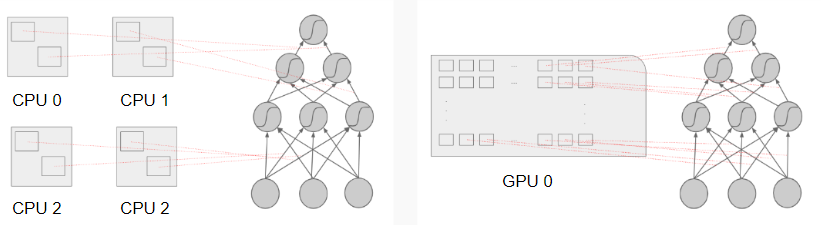
\includegraphics{figure/cpu_gpu.png}}
      \caption{\textit{Left:} Each CPU can do 2-8 parallel computations. \textit{Right:} A single GPU can do thousands of simple parallel computations.}
  \end{figure}
\end{frame}

\begin{frame} {Graphics Processing Units (GPUs)}
  \begin{itemize}
    \item Initially developed to accelerate the creation of graphics
    \item Massively parallel: identical and independent computations for every pixel
    \item Computer Graphics makes heavy use of linear algebra (just like neural networks)
    \item Less flexible than CPUs: all threads in a core concurrently execute the same instruction on different data.
    \item Very fast for CNNs, RNNs need more time
    \item Popular ones: GTX 1080 Ti, RTX 3080 / 2080 Ti, Titan RTX, Tesla V100 / A100
    \item Hundreds of threads per core, few thousands cores, around 10 teraFLOPS in single precision, some 10s GBs of memory
    \item Memory is important - some SOTA architectures do not fit GPUs with <10 GB  
  \end{itemize}
\end{frame}

\begin{frame} {Tensor Processing Units (TPUs)}
  \begin{itemize}
    \item Specialized and proprietary chip for deep learning developed by Google
    \item Hundreds of teraFLOPS per chip
    \item Can be connected together in \emph{pods} of thousands TPUs each (result: hundreds of \textbf{peta}FLOPS per pod)
    \item Not a consumer product! Can be used in the Google Cloud Platform (from 1.35 USD / TPU / hour) or Google Colab (free!)
    \item Enables DeepMind to make impressive progress : AlphaZero for Chess became world champion after just 4 hours of training concurrently on 5064 TPUs
  \end{itemize}
\end{frame}

\begin{frame} {And everything else...}
  \begin{itemize}
    \item With such powerful devices, memory/disk access during training become the bottleneck
    \begin{itemize}
      \item Nvidia DGX-1: Specialized solution with eight Tesla V100 GPUs, dual Intel Xeon, 512 GB of RAM, 4 SSD disks of 2TB each
    \end{itemize}
    \item Specialized hardware for on-device inference
    \begin{itemize}
      \item Example: Neural Engine on the Apple A11 (used for FaceID)
      \item Keywords/buzzwords: \emph{Edge computing} and \emph{Federated learning}
    \end{itemize}
  \end{itemize}
\end{frame}

%%%%%%%%%%%%%%%%%%%%%%%%%%%%%%%%%%%%%%%%%%%%%%%%%%%%%%%%%%%%%%%
\section{Software for Deep Learning}
\begin{frame} {Software for Deep Learning}
  \begin{itemize}
    \item CUDA is a very \textit{low level} programming language and thus writing code for deep learning requires a lot of work.
    \item Deep learning (software) frameworks:
    \begin{itemize}
      \item Abstract the hardware (same code for CPU/GPU/TPU)
      \item Automatically differentiate all computations
      \item Distribute training among several hosts
      \item Provide facilities for visualizing and debugging models
      \item Can be used from several programming languages
      \item Based on the concept of \emph{computational graph}
    \end{itemize}
  \end{itemize}
  \begin{figure}
    \centering
    \scalebox{0.25}{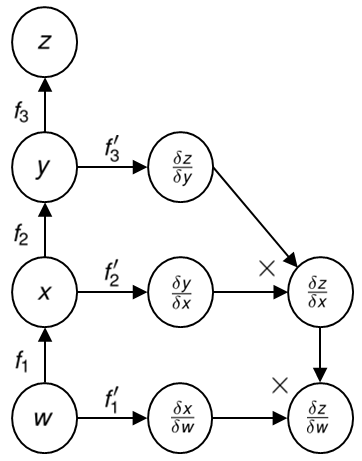
\includegraphics{figure/compgraph3}}
  \end{figure}
\end{frame}

\begin{frame} {Software for Deep Learning}
  \begin{wrapfigure}{R}{0.3\textwidth}
    \centering
      \scalebox{0.3}{
\includegraphics{figure/tflow.png}}
  \end{wrapfigure}
\textbf{Tensorflow}
\begin{itemize}
  \item Popular in the industry
  \item Developed by Google and \newline open source community
  \item Python, R, C++ and Javascript APIs
  \item Distributed training on GPUs and TPUs
  \item Tools for visualizing neural nets, running them efficiently on phones and embedded devices.
\end{itemize}

\begin{wrapfigure}{R}{0.3\textwidth}
  \centering
  \scalebox{0.3}{
\includegraphics{figure/keras.png}}
\end{wrapfigure}

\textbf{Keras}
  \begin{itemize}
    \item Intuitive, high-level \textbf{wrapper} on Tensorflow for rapid prototyping
    \item Python and (unofficial) R APIs
    
  \end{itemize}
\end{frame}

\begin{frame} {Software for Deep Learning}
  \begin{wrapfigure}{R}{0.3\textwidth}
    \centering
      \scalebox{0.3}{
\includegraphics{figure/pytorch.png}}
  \end{wrapfigure}

\textbf{Pytorch}
  \begin{itemize}
    \item Popular in academia
    \item Supported by Facebook
    \item Python and C++ APIs
    \item Distributed training on GPUs
  \end{itemize}

  \begin{wrapfigure}{R}{0.3\textwidth}
    \centering
      \scalebox{0.3}{
\includegraphics{figure/mxnet.png}}
  \end{wrapfigure}
  \vspace{3mm}
  \textbf{MXNet}
    \begin{itemize}
      \item Open-source deep learning framework written in C++ and cuda (used by Amazon for their Amazon Web Services) 
      \item Scalable, allowing fast model training
      \item Supports flexible model programming and multiple languages (C++, Python, Julia, Matlab, JavaScript, Go, \textbf{R}, Scala, Perl)
    \end{itemize}
\end{frame}

%%%%%%%%%%%%%%%%%%%%%%%%%%%%%%%%%%%%%%%%%%%%%%%%%%%%%%%%%%%%%%%%%%
\section{Example: MNIST digit recognizer}
\begin{vbframe}{MNIST digit recognizer}
  \begin{itemize}
    \item The MNIST dataset is a large dataset of handwritten digits (black and white) that is commonly used for benchmarking various image processing algorithms.
    \item It is a good dataset for people who want to try learning techniques and pattern recognition methods on real-world data while spending minimal effort on preprocessing and formatting.
    \item  There have been a number of scientific papers on attempts to achieve the lowest error rate. One paper, using a hierarchical system of convolutional neural networks (chapter 5), manages to get an error rate of only 0.23 percent.
  \end{itemize}

\framebreak
  \begin{figure}
    \centering
      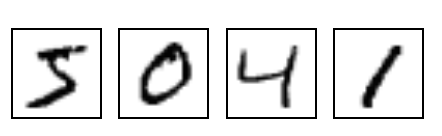
\includegraphics[width=10cm]{figure/mnist.png}
      \caption{Snipped from the mnist data set (LeCun and Cortes (2010)).}
  \end{figure}
  \begin{itemize}
    \item 70k image data of handwritten digits with $28 \times 28$ pixels.
    \item Classification task with 10 classes (0, 1, 2, ..., 9).
  \end{itemize}

%%%%%%%%%%%%%%%%%%%%%%%%%%%%%%%%%%%%%%%%%%%%%%%%%%%%%%%%%%%%%%%%%%%%%%%%
%%%%%%%%%%%%%%%%%%%%%%%%%%%%%% READ ME!!! %%%%%%%%%%%%%%%%%%%%%%%%%%%%%%
%%%%%%%%%%%%%%%%%%%%%%%%%%%%%%%%%%%%%%%%%%%%%%%%%%%%%%%%%%%%%%%%%%%%%%%%
% The following slides include lots of code chunks which have been     %
% temporarily disabled (eval = FALSE, echo = FALSE) and replaced by    %
% screenshots of the corresponding outputs (to maintain colorization). %
% Else, one would need a working version of mxnet (and a fast CPU/GPU) %
% to compile the code in a finite amount of time.                      %
%%%%%%%%%%%%%%%%%%%%%%%%%%%%%%%%%%%%%%%%%%%%%%%%%%%%%%%%%%%%%%%%%%%%%%%%


\framebreak
  \begin{minipage}{0.45\textwidth}
    \begin{itemize}
      \item We attempt classification with the model on the right:
    \end{itemize}
  \end{minipage}
  \begin{minipage}{0.45\textwidth}
    \begin{figure}
      \centering
        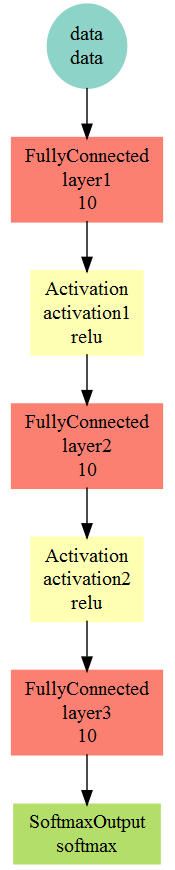
\includegraphics[width=1.5cm]{figure/mxnet_codechunk_4b.png}
    \end{figure}
  \end{minipage}



\framebreak
  \begin{itemize}
    \item We used SGD with a minibatch of size 100 and trained for 10 epochs.
    \item Consequently we feed our algorithm successively with 100 training samples before updating the weights.
    \item After 10 epochs, our neural network begins to stagnate at a training accuracy of roughly $93.5\%$
    \item Next, we use the model to predict the test data.
    \item We find that the accuracy of the model on the test data is only $89.843\%$ which is unsatisfactory. 
  \end{itemize}
  
\framebreak
  \begin{minipage}{0.45\textwidth}
    \begin{itemize}
      \item Because the performance of the previous model was somewhat poor, we try the following, much larger, network (all other parameters remain the same)
      \item Rerunning the training with the new architecture, this model yields us a training accuracy of $99.39\%$ and a test accuracy of $96.514\%$.
    \end{itemize}
  \end{minipage}
  \begin{minipage}{0.45\textwidth}
    \begin{figure}
      \centering
        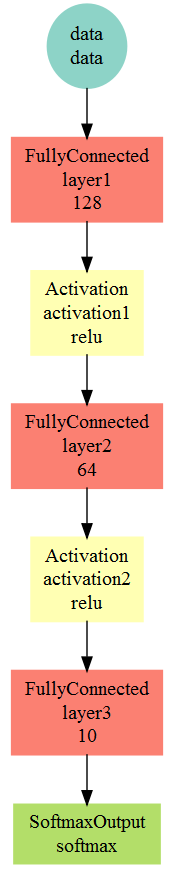
\includegraphics[width=1.5cm]{figure/mxnet_codechunk_10.png}
    \end{figure}
  \end{minipage}
\end{vbframe}

\begin{frame} {Key hyperparameters}
  \begin{itemize}
    \item In addition to the structure/topology of the neural network, the performance of a model is also strongly affected by some key hyperparameters such as:
      \begin{itemize}
        \item $\alpha$, the learning rate
        \item $\lambda$, the regularization coefficient
        \item $T$, the number of training iterations
        \item $m$, the minibatch size
        \item and others...
      \end{itemize}
    \item These hyperparameters typically control the complexity of the model and the convergence of the training algorithm.
    \item In the next couple of lectures, we'll examine methods and techniques to set these hyperparameters and the theoretical motivations behind many of them.
  \end{itemize}
\end{frame}

%%%%%%%%%%%%%%%%%%%%%%%%%%%%%%%%%%%%%%%%%%%%%%%%%%%%%%%%%%%%%%%%%%
%%%%%%%%%%%%%%%%%%%%%%%%%%%%%%%%%%%%%%%%%%%%%%%%%%%%%%%%%%%%%%%%%%
%%%%%%%%%%%%%%%%%%          REFERENCES          %%%%%%%%%%%%%%%%%%
%%%%%%%%%%%%%%%%%%%%%%%%%%%%%%%%%%%%%%%%%%%%%%%%%%%%%%%%%%%%%%%%%%

%\section{References}

\begin{vbframe}
\frametitle{References}
\footnotesize{
\begin{thebibliography}{99}

%%%%%%%%%%%%%%%%%%%%%%%%%%%%%%%%%%
\bibitem[Yann LeCun and Corinna Cortes, 2010]{2} Yann LeCun and Corinna Cortes (2010)
\newblock MNIST handwritten digit database
\newblock \emph{\url{http://yann.lecun.com/exdb/mnist/}}
%%%%%%%%%%%%%%%%%%%%%%%%%%%%%%%%%%
\end{thebibliography}
}
\end{vbframe}

\endlecture
\end{document}